% ====================================================================
% Section 7 (v2): The applicability condition - tube/sp.
% Faithful to experiments/sweep_topologies.py + analyze_sweep.py output.
% This is the strongest standalone result: r=0.778, p=0.0006.
% ====================================================================
\section{When Physics Wins, Loses, or Ties: a Topological Condition}
\label{sec:applicability}

The equivalence of Sections~\ref{sec:equivalence}--\ref{sec:fair} is not
uniform. On some topologies the physical core has room to spread load and does
well; on others---notably the real WAN backbones---it does not. A result that
holds ``most of the time'' is only half a result unless one can say \emph{when}
it holds. This section supplies that condition, and it turns out to be a simple
property of the topology, computable in advance and independent of any router.

\subsection{The tube/sp ratio}

For a source--destination pair, consider the set of edges lying on paths only
mildly longer than the shortest one---the ``tube'' of near-shortest routes
within a small length tolerance of the shortest-path length. Define the
\textbf{tube/sp ratio} of a topology as the mean, over demand pairs, of the
number of edges in that tube divided by the shortest-path length. Intuitively
it measures \emph{room to manoeuvre}: how many viable alternative routes exist
near the shortest path. A grid has a high tube/sp---many equivalent detours; a
sparse backbone has a low one---few alternatives that are not far longer.

Crucially, tube/sp is a property of the graph and the demand alone. It does not
mention EMMET, CONGA, or any routing algorithm. It can be computed before a
single packet is sent.

\subsection{It predicts the advantage}

We computed tube/sp for all 15 topologies and regressed the physical core's
relative loss reduction (versus CONGA) against it (Table~\ref{tab:tube},
Figure~\ref{fig:tube}).

\begin{figure}[t]
\centering
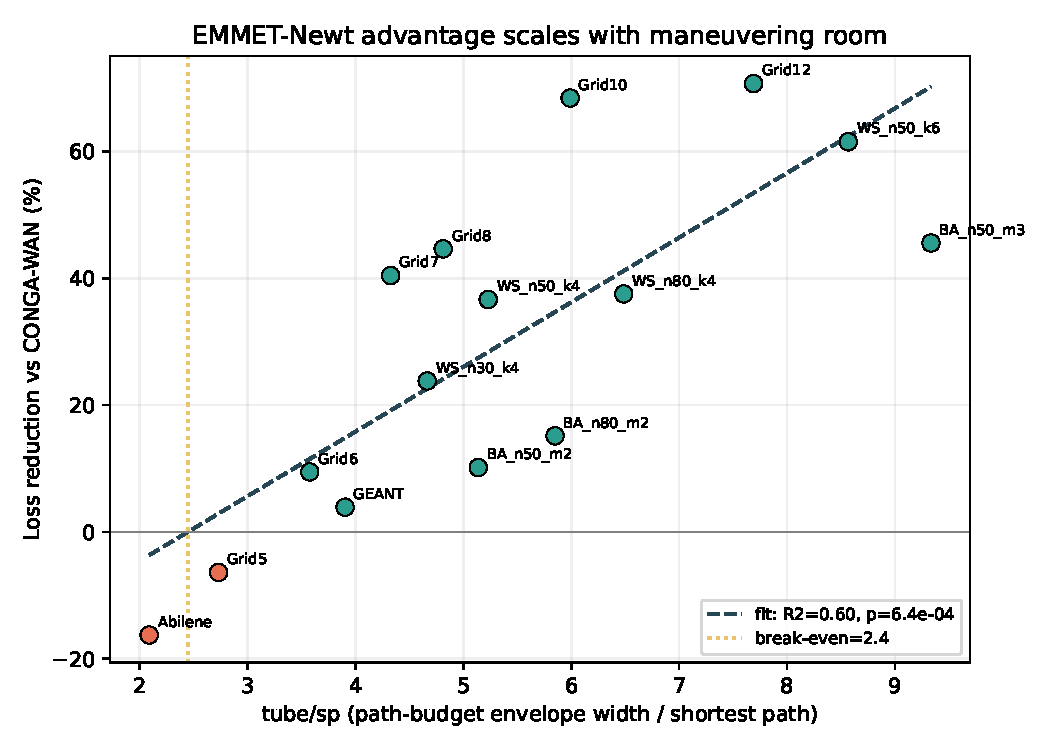
\includegraphics[width=0.8\linewidth]{figure_tube_sweep.pdf}
\caption{Relative loss reduction of the two-term core versus CONGA as a function of the topology tube/sp ratio (15 topologies). Fit: reduction\%=10.2(tube/sp)-25.0, Pearson $r=0.78$, $p=0.0006$, break-even near 2.45. Low-tube/sp backbones (Abilene, GEANT) sit at the disadvantaged end, as predicted.}
\label{fig:tube}
\end{figure}


\begin{figure}[t]
\centering
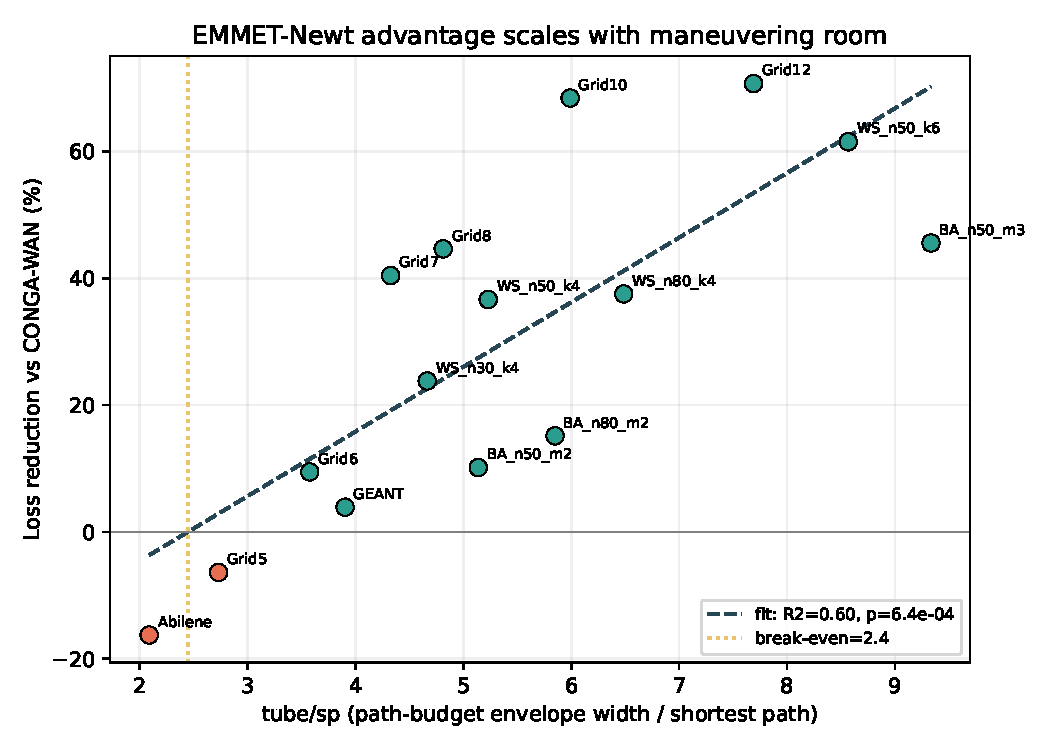
\includegraphics[width=0.8\linewidth]{figure_tube_sweep.pdf}
\caption{Relative loss reduction of the two-term physical core versus CONGA as
a function of the topology's tube/sp ratio, across 15 topologies. The fit is
$\text{reduction\%}=10.2\cdot(\text{tube/sp})-25.0$ (Pearson $r=0.78$,
$p=0.0006$), with break-even near tube/sp $=2.45$. Low-tube/sp real backbones
(Abilene, G\'EANT) sit at the disadvantaged end, as predicted.}
\label{fig:tube}
\end{figure}

\begin{table}[t]
\centering
\caption{Relative loss reduction of the physical core versus CONGA, ordered by
the topology's tube/sp ratio. Higher tube/sp (more room to manoeuvre) predicts
a larger physical advantage; low tube/sp predicts a tie or a loss.}
\label{tab:tube}
\small
\begin{tabular}{lrr}
\toprule
Topology & tube/sp & reduction\% \\
\midrule
Abilene      & 2.09 & $-16.3$ \\
Grid $5$     & 2.73 & $-6.4$ \\
Grid $6$     & 3.58 & $+9.5$ \\
G\'EANT      & 3.90 & $+3.9$ \\
Grid $7$     & 4.33 & $+40.4$ \\
WS $n30\,k4$ & 4.67 & $+23.8$ \\
Grid $8$     & 4.81 & $+44.6$ \\
BA $n50\,m2$ & 5.14 & $+10.1$ \\
WS $n50\,k4$ & 5.23 & $+36.7$ \\
BA $n80\,m2$ & 5.85 & $+15.1$ \\
Grid $10$    & 5.99 & $+68.4$ \\
WS $n80\,k4$ & 6.49 & $+37.5$ \\
Grid $12$    & 7.69 & $+70.7$ \\
WS $n50\,k6$ & 8.57 & $+61.5$ \\
BA $n50\,m3$ & 9.33 & $+45.6$ \\
\bottomrule
\end{tabular}
\end{table}

The relationship is strong and significant:

\begin{itemize}
\item Pearson $r = 0.78$ ($p = 0.0006$), Spearman $\rho = 0.82$
($p = 0.0002$).
\item Linear fit: $\text{reduction\%} = 10.2 \cdot (\text{tube/sp}) - 25.0$,
with $R^2 = 0.60$.
\item Break-even at $\text{tube/sp} \approx 2.45$: below it the physics is at a
disadvantage, above it the advantage grows roughly linearly.
\end{itemize}

The two real backbones sit exactly where the metric says they should. Abilene
(tube/sp $=2.09$) is below break-even and is the one topology where the core
clearly loses; G\'EANT (tube/sp $=3.90$) is just above it and lands on a
near-tie ($+3.9\%$). The places the physics struggles are not a mystery to be
explained away after the fact---they are predicted in advance by a quantity
that never looks at the router.

\subsection{Why this matters}

This converts the contribution from an observation into a predictor. We are not
claiming that classical physics always matches engineered routing; we are
claiming something more precise and more useful: that it does so exactly when
the topology offers enough near-shortest alternatives for a local gradient rule
to exploit, and that the threshold is measurable. A network operator could
compute tube/sp for their topology and know, before deployment, whether a
two-term physical router would be competitive on it.

It also explains the historical arc of this project. The early, headline result
was measured on G\'EANT against a weak baseline; G\'EANT's middling tube/sp
($3.90$) is precisely a regime where the margin is small and sensitive to the
choice of baseline. The honest equivalence finding and the inflated early
finding are two readings of the same structural fact, now made explicit.

\subsection{Caveats}

$R^2 = 0.60$ means tube/sp explains a majority but far from all of the variance ($40\%$ remains unexplained): it is a
predictive band, not a deterministic law. The scale-free (Barab\'asi--Albert)
points are the loosest fit, sitting below the regression line---their hub
structure concentrates load in ways the tube measure, which averages over
pairs, does not fully capture. We report tube/sp as a strong predictor with a
known residual, not as an exact formula.


\begin{figure}[t]
\centering
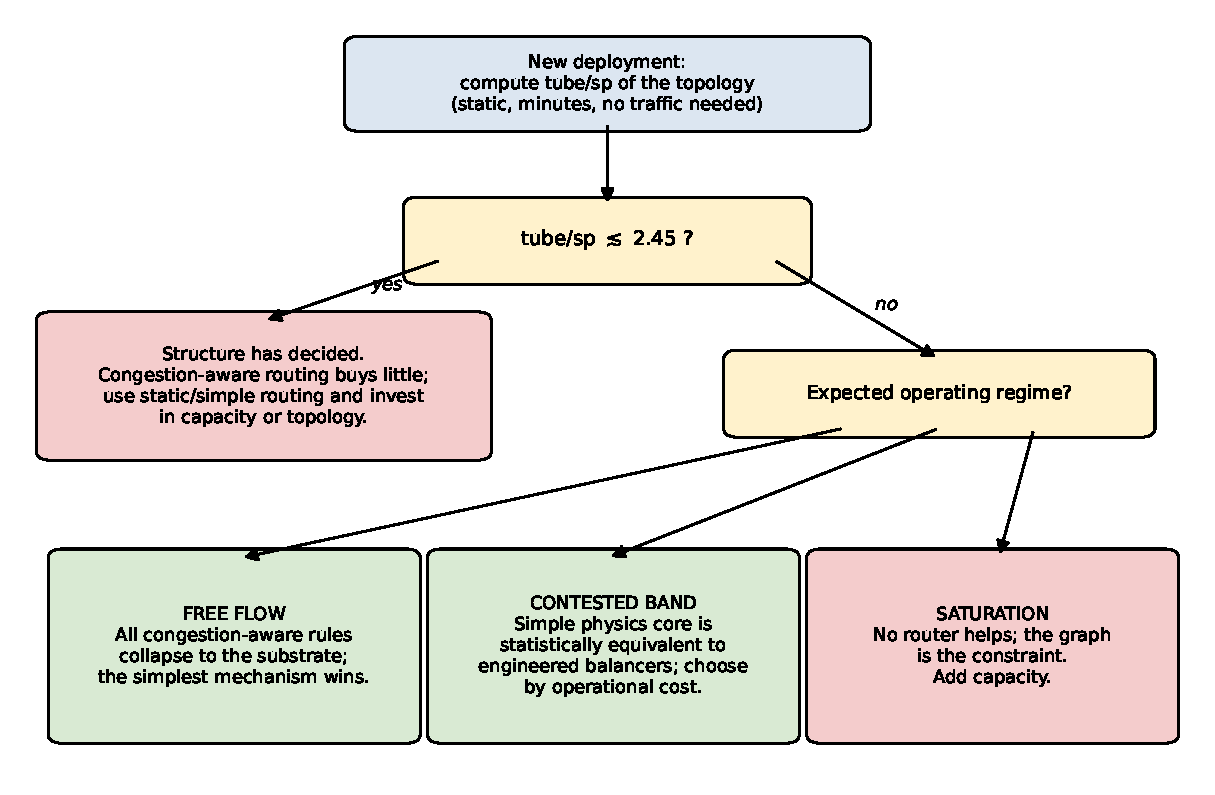
\includegraphics[width=0.92\columnwidth]{figs/operator_decision.pdf}
\caption{The two-factor law as a pre-deployment decision diagram. The
structural ratio tube/sp is computable from topology alone, before any
traffic exists; the break-even $\approx 2.45$ and the regime boundaries
are the bench estimates of Sections~\ref{sec:twofactor}
and~\ref{sec:leverage}.}
\label{fig:operator}
\end{figure}
